\section{Project Description}

\subsection{Motivation}
Industrialization and climate-change go hand in hand in affecting air quality.
Industrialization worsens climate change and air quality, and climate change
further worsens air quality through natural disasters such as wildfires, acid
rain, or sand storms. It is estimated that 7 million people die from air
pollution globally a year \cite{interplay-climate-change-air-pollution-health}.
Wildfires pose a significant risk for the general population, and especially
those at risk for respiratory infections and people over the age of 65. There is
also a disproportionate increase in air pollution for those in poorer
communities where often times they are close to industrial areas
\cite{socioeconomic-disparities-air-pollution-review}. By providing a low-cost
way of measuring the overall air quality, people can be more educated about the
air quality in their communities, and provide them with the data to back up
their complaints to their local municipalities. For developing countries, they
might be less focused on the environment due to cost constraints, but by
providing a cheap option for measuring air pollution, they can potentially make
more educated decisions about where to make improvements. A low cost air quality
sensor might also be of interest for those that are health conscience, or are
already at risk for respiratory disease, as they can make decisions based on the
current air quality. People living in cities, or other highly industrialized
areas, are also subject to increased air pollution, mostly from motor vehicles
(what create smog and haze), and from factories. Even short term exposure can
cause adverse health affects \cite{health-impacts-air-pollution-review}.
However, the full extent of long term exposure to these pollutants is
inconclusive. What is conclusive is that air pollution is the cause for millions
of deaths world wide each year.

Air quality sensors are very valuable for people living in areas that are high
risk for wildfires, such as California. Smoke from wildfires can be deadly, if
not cause serious health effects depending on the smoke concentration and
exposure time. Based on the air quality, using either the AQI or the AirNow
index, people might need to stay indoors. Another potential use case of an air
quality sensor is the ability to detect wildfire by deploying them to
wildfire-prone areas. By using LoRa, these sensors can provide a wide range of
coverage centered around a LoRa gateway.


\subsection{Goals and Objectives}
\begin{itemize}
    \item The sensor nodes should be low cost. 
    \item The sensor nodes should be lightweight. 
    \item The sensor nodes should be able to read data from the sensors and transmit that data to a LoRa gateway. 
    \item The sensors nodes should be able to communicate over a large enough distance in order to make it feasible to cover large enough area with nodes.
    \item The nodes should require little to no maintenance.
    \item The sensor nodes should be easy to install.
    \item The gateway should be able to connect to the internet to send the data it receives from the nodes to an external server over the internet.
\end{itemize}


\subsection{Requirements Specifications}
\begin{table}[H]
\centering
\caption{The gateway requirements}
\begin{tabularx}{\linewidth}{|c|X|c|c|}
\hline
No. & Requirement & Value & Units \\
\hline\hline
1.0 & The gateway should cost no more than \$200 & 200 & dollars \\\hline
1.1 & The gateway should be no larger than 24" x 24" x 24" & 24x24x24 & inches \\\hline
1.2 & The gateway weight should be no more than than 10 pounds & 10 & lbs \\\hline
1.3 & The gateway should utilize LoRaWAN with the base station as the gateway with the capacity to connect with up to 8 devices simultaneously. & 8 & nodes \\\hline
1.4 & The gateway should be able to communicate with nodes up to 10 km away with ideal conditions & 10	& km \\\hline
1.5 & The gateway should be able to communicate with nodes up to 3 km away in an urban environment & 3 & km \\\hline
1.6 & The gateway should be able to manage up to 256 nodes & 256 & nodes \\\hline
\end{tabularx}
\label{tab:networkingRequirements}
\end{table}

\begin{table}[H]
\centering
\caption{The sensor node requirements.}
\begin{tabularx}{\linewidth}{|c|X|c|c|}
\hline
No. & Requirement & Value & Units \\
\hline\hline
2.0 & The sensor node should cost no more than \$150 & 150 & dollars \\\hline
2.1 & The sensor node should be no larger than 12" x 12" x 12" & 12x12x12 & inches \\\hline
2.2 & The sensor node weight should be no more than 10 pounds & 10 & lbs \\\hline
2.3 & The sensor node should stay operational without intervention for 1 year & 1 & year \\\hline
2.4 & The sensor node sensors should have a maximum tolerance of +/- 20\% & 20 & \% \\\hline
2.5 & The sensor node should transmit for no more than 30 seconds every 24 hours & 30 & seconds \\\hline
\end{tabularx}
\label{tab:nodeRequirements}
\end{table}

\begin{table}[H]
\centering
\caption{The gateway and networking engineering specifications}
\begin{tabularx}{\linewidth}{|c|X|}
\hline
No. & Requirement \\
\hline\hline
3.0 & The gateway shall use LoRa and LoRaWAN for the wireless communication protocol \\\hline
3.1 & The gateway should adhere to the LoRa Fair Access policy \\\hline
3.2 & The gateway should have enough internet bandwidth to support all of its connected nodes \\\hline
3.3 & The network shall utilize a star networking topology.\\\hline
3.4 & We define a component of our network to be known as a cell, which shall consist of nodes connected to a gateway. \\\hline
3.5 & The gateway shall be able communicate with an external server over the internet.\\\hline
3.6 & The server shall be hosted on existing web hosting platform.\\\hline
3.7 & The server shall host a website that displays data collected from the sensors.\\\hline
\end{tabularx}
\label{tab:networkingSpecs}
\end{table}

\begin{table}[H]
\centering
\caption{The node engineering specifications}
\begin{tabularx}{\linewidth}{|c|X|}
\hline
No. & Requirement \\
\hline\hline
4.0 & The sensor node shall use a radio and antenna that is part of a daughterboard that can be attached to the main PCB.\\\hline
4.1 & The node should use a battery and solar panel \\\hline
4.2 & The sensor node shall contain a microcontroller. \\\hline
4.3 & The sensor node microcontroller shall support the UART protocol.\\\hline
4.4 & The sensor node microcontroller shall have at least one ADC.\\\hline
4.5 & The sensor node microcontroller shall support JTAG debugging.\\\hline
4.6 & The sensor node shall contain a NO2 sensor.\\\hline
4.7 & The sensor node shall contain a PM sensor.\\\hline
4.8 & The sensor node shall contain a SO2 sensor.\\\hline
4.9 & The sensor node shall contain a O3 sensor.\\\hline
4.10 & The sensor node shall contain a CO sensor.\\\hline
\end{tabularx}
\label{tab:nodeSpecs}
\end{table}

\begin{table}[H]
\centering
\caption{The constraints.}
\begin{tabularx}{\linewidth}{|X|}
\hline
Constraint \\
\hline
The nodes must be light enough so that they can be affixed to a building or other structure and not be of a concern to fall off.\\\hline
The nodes must low cost to be able to placed in greater number. \\\hline
The nodes must be able to withstand water from rainfall.\\\hline
The nodes must be able to withstand high winds. \\\hline
The nodes must be able to withstand temperature extremes. \\\hline
The nodes must be able to support a communication range of at least 1 km\\\hline
The nodes must be able to operate on less power than what one solar panel could generate in a single day to allow for operation when there is no sunlight present.\\\hline
The gateway must be able to operate off of mains power.\\\hline
\end{tabularx}
\label{tab:constraints}
\end{table}

\subsection{House of Quality}
In Figure \ref{fig:hoq}, we provide a comparison between our marketing parameters and our engineering requirements. The marketing parameters are qualitative in nature and are chosen based on the qualities that we imagine customers would be looking for in this product. Light refers to the node having a low weight. Accurate means that the sensors produce a reading that reflects the correct concentration of gases in the air around the node. It could also refer to having enough nodes to cover an area to provide a high resolution of sensor data. Low maintenance and reliable are somewhat related parameters, however, low maintenance refers to the ability of the node to operate for a long enough period of time without needing to replace various components and reliable refers to the ability of the node to survive the outdoor elements and continue to provide quality sensor data over time. Real time means that the node should be transmitting and reading data from its sensors as often as possible. Easy to install means that the nodes should be able to placed in the desired location with minimal effort. Ideally, the nodes would be able to be placed in wide variety of situations and locations with relative ease.

In contrast to the marketing parameters, the engineering requirements are quantitative in nature. Battery life is key since it determines how long the nodes can be deployed without having to have batteries replaced or recharged. Node-to-gateway distance refers to how far away a node can be away from a gateway and is a critical requirement because it directly impacts how large of and area you can cover with nodes. The number of nodes per gateway is also important because we would like to minimize the number of gateways required for any given number of nodes in the network. Sensor accuracy refers specifically to how far the true measurement of a given gas is from the value outputted by the sensor. It is given as a $\pm$percentage. Finally, the nodes should of course be as small, light, and cost as little as possible.
\begin{figure}[tbh]
    \centering
    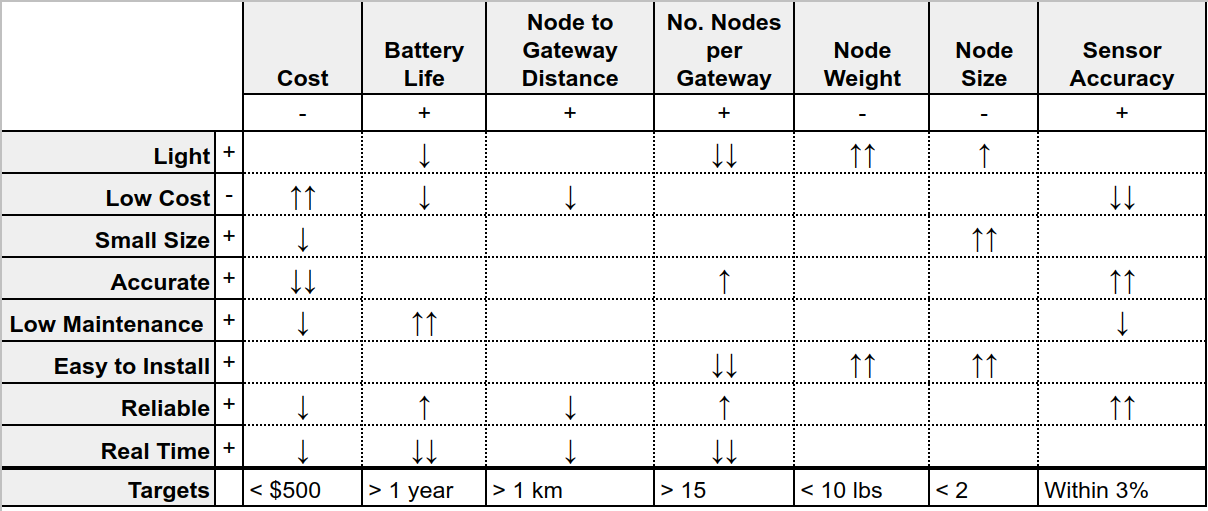
\includegraphics[width=6.25in]{./figures/hoq.png} 
    \caption{The house of quality diagram.}
    \label{fig:hoq}
\end{figure}

% \subsection{Similar Existing Products}
%     \subsubsection{Product 1}
%     \subsubsection{Product 2}

